\section{Blockchain-Technologie}
\label{sec:blockchain_basics}

%Als Grundlage für Blockchains dient die \textit{Distributed Ledger Technology} (DLT). Was alle DLTs gemeinsam haben, ist, dass die Daten auf allen Teilnehmern des Netzwerkes gespeichert werden und die Verwendung von kryptografischen Technologien, wie Hash-Funktionen und Konsensmechanismen \parencite{Ioini_DLTReview}.

%Bei der DLT handelt es sich um eine Technologie, die es ermöglicht, Daten in einem dezentralen Netzwerk zu speichern. Die Daten werden dabei auf allen Teilnehmern des Netzwerkes gespeichert. Dadurch ist es nicht möglich, die Daten zu manipulieren, da die Daten auf allen Teilnehmern des Netzwerkes gespeichert sind. Wenn ein Teilnehmer versucht, die Daten zu manipulieren, wird dies von den anderen Teilnehmern bemerkt und die manipulierten Daten werden nicht akzeptiert \parencite[S. 10]{Fill_BlockchainGrundlagen}.

Christoph Meinel und Tatiana Gayvoronskaya beschreiben die Blockchain-Technologie in ihrem Buch \textit{Blockchain - Hype oder Innovation} wie folgt:

\begin{quote}
    \textit{Die Innovation der Blockchain-Technologie ist weder ein neuer Verschlüsselungsalgorithmus
    noch eine „Alientechnologie“, sondern eine erfolgreiche Kombination bereits
    vorhandener technologischen Ansätze wie Kryptografie, dezentrale Netzwerke und Konsensfindungsmodelle.}\parencite[S. 17]{Meinel_BlockchainHypeInnovation}
\end{quote}

\noindent Daraus ergibt sich die Frage, was Blockchain eigentlich ist und wie die bereits vorhandenen technologischen Ansätze miteinander vereint werden. Diese Fragen werden in diesem Kapitel beantwortet. Zunächst wird der Begriff Blockchain definiert und anschließend die Funktionsweise erläutert. Daraufhin werden die Konsensmechanismen Proof-of-Work und Proof-of-Stake vorgestellt. Abschließend wird auf die Sicherheit von Blockchain eingegangen und Angriffe auf Blockchain werden erläutert.
% #TODO: Distributed Ledger als Vorgänger zu Blockchain erwähnen?

\subsection{Definition von Blockchain}
\label{subsec:blockchain_definition}

Der Begriff \textit{Blockchain} setzt sich aus den englischen Wörtern \textit{block} (Block) und \textit{chain} (Kette) zusammen. Eine Blockchain ist also eine Kette von Blöcken. Wie in Abbildung \ref{fig:blockchain} zu sehen ist, beinhaltet ein Block den Block-Header und mehrere Transaktionen. 

\begin{figure}[H]
    \centering
    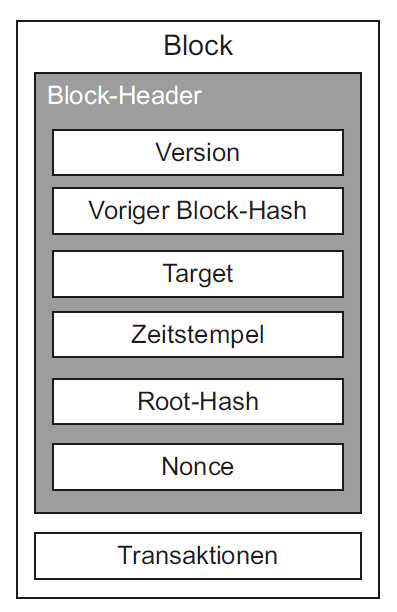
\includegraphics[width=0.4\linewidth]{images/blockchain_block.png}
    \caption{Aufbau eines Blocks \parencite[S. 11]{Fill_BlockchainGrundlagen}}
    \label{fig:blockchain}
\end{figure}


\noindent Der Block-Header enthält Informationen über den Block, wie zum Beispiel den Hash des vorherigen Blocks, die Schwierigkeit, den Zeitstempel und die Nonce. Die Schwierigkeit wird durch das \textit{Target}-Feld angegeben und beschreibt, wie schwer es ist, das kryptografische Puzzle zu lösen und damit auch wie schwer es ist, einen neuen Block an die Blockchain anzuhängen. Die Suche nach der Lösung dieses Puzzles wird auch als \textit{Mining} bezeichnet. Der erste, der das Puzzle löst, präsentiert als Beweis dieser Lösung die sogenannte \textit{Nonce}. Nachdem diese neue Version der Blockchain (mit dem neu angehängten Block) an alle anderen Teilnehmer verteilt wurde, kann jeder Teilnehmer überprüfen, ob die Lösung korrekt ist. Die Nonce ist eine zufällige Zahl, die bei der Lösung des Puzzles verwendet wird und aufwändig zu berechnen ist. Durch den Verweis im Block-Header auf den vorherigen Block entsteht eine Kette von Blöcken (siehe Abbildung \ref{fig:chain_of_blocks}), die \textit{Blockchain} genannt wird \parencite[S. 10-12]{Fill_BlockchainGrundlagen}.

\begin{figure}[H]
    \centering
    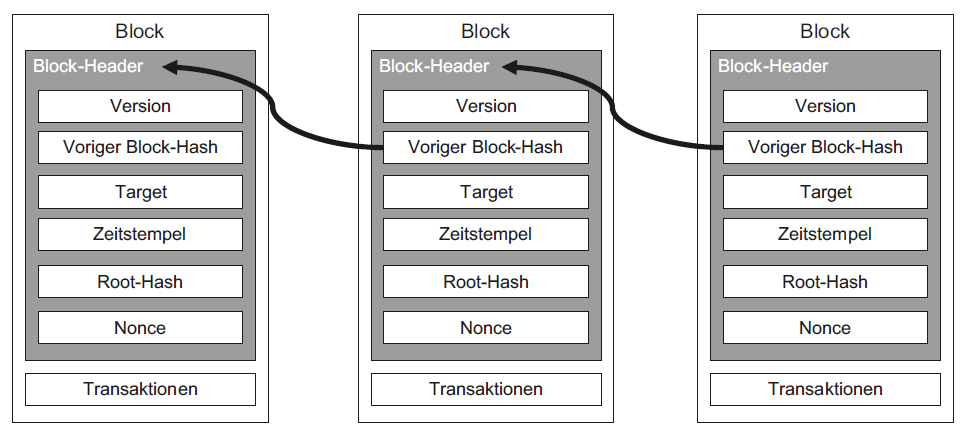
\includegraphics[width=0.9\linewidth]{images/chain_of_blocks.png}
    \caption{Kette aus Blöcken \parencite[S. 12]{Fill_BlockchainGrundlagen}}
    \label{fig:chain_of_blocks}
\end{figure}

% Die Transaktionen enthalten jeweils Informationen zum Sender, dem Empfänger und dem Betrag.


\subsection{Kryptografische Grundlagen}
Aus der Kryptografie werden Hash-Funktionen, kryptografische Puzzles, Hash-Bäume und digitale Signaturen verwendet. Hash-Funktionen können dazu verwendet werden, um die Integrität von Daten zu gewährleisten. Eine Hash-Funktion bildet eine beliebig lange Eingabe auf eine feste Länge ab. Kryptografische Hash-Funktionen sind Hash-Funktionen, die bestimmte Eigenschaften erfüllen müssen. Die beiden wichtigsten Eigenschaften sind die \textit{Einwegfunktion} und die \textit{Kollisionsresistenz}. Eine Hash-Funktion erfüllt die Eigenschaft der Einwegfunktion, wenn es nicht möglich ist, von der Ausgabe auf die Eingabe zu schließen. Das bedeutet, dass es nicht möglich ist, aus dem Hash-Wert die ursprünglichen Daten zu rekonstruieren. Die Eigenschaft der \textit{Kollisionsresistenz} ist erfüllt, wenn es nicht möglich ist, zwei verschiedene Eingaben zu finden, die auf den gleichen Hash-Wert abgebildet werden \parencites[S. 12-13]{Brünnler_BlockchainKurzGut}[S. 6]{Fill_BlockchainGrundlagen}.

Kryptografische Puzzles werden dazu verwendet, um die Schwierigkeit beim Mining zu erhöhen. Dabei soll mittels Hash-Funktionen ein bestimmter Ausgabewert gefunden werden. Laut Definition der Einwegfunktion ist es nicht möglich, von der Ausgabe auf die Eingabe zu schließen. Daher kann die gesuchte Eingabe nur durch Ausprobieren gefunden werden. Die Schwierigkeit kann durch die Anzahl der Nullen, die am Anfang des Hash-Wertes stehen müssen, angegeben werden. Je mehr Nullen am Anfang des Hash-Wertes stehen müssen, desto schwieriger ist es, die Lösung zu finden, da dadurch der Lösungsraum verkleinert wird \parencite[S. 6-7]{Fill_BlockchainGrundlagen}.

Ein \textit{Merkle-Baum} ist ein binärer Baum, bei dem jeder Knoten den Hash-Wert seiner Kinder enthält. Der nach seinem Erfinder Ralph Merkle benannten Hash-Baum wird in der Blockchain zum Aufbau von Datenstrukturen verwendet. Der Hash-Wert der Wurzel des Baumes wird auch als \textit{Root-Hash} oder \textit{Merkle-Root} bezeichnet. Wenn sich ein Blatt des Baumes ändert, ändert sich auch der Hash-Wert der Wurzel. Dadurch kann überprüft werden, ob sich die Daten geändert haben. Wenn sich die Daten geändert haben, ändert sich auch der Root-Hash. Wenn sich die Daten nicht geändert haben, bleibt der Root-Hash gleich. Dadurch kann die Integrität der Daten überprüft werden \parencite[S. 7-8]{Fill_BlockchainGrundlagen}. In Abbildung is der Aufbau eines Merkle-Baumes zu sehen.

\begin{figure}[H]
    \centering
    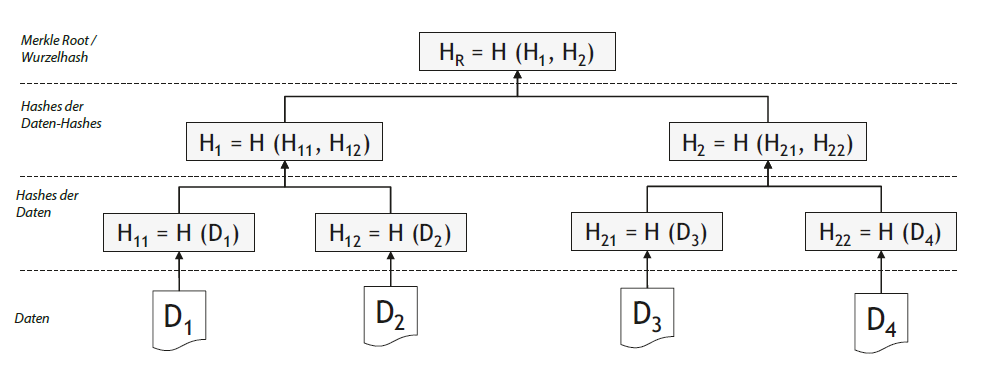
\includegraphics[width=0.9\linewidth]{images/merkle_tree.png}
    \caption{Aufbau eines Merkle-Baumes \parencite[S. 8]{Fill_BlockchainGrundlagen}}
    \label{fig:merkle_tree}
\end{figure}

\noindent Von jedem Dokument $D_{1}$, $D_{2}$, $D_{3}$ und $D_{4}$ wird ein Hash-Wert berechnet und in einem Blatt des Baumes gespeichert. Die Hash-Werte der Blätter werden dann paarweise gehasht und in den Knoten darüber gespeichert. Dieser Vorgang wird solange wiederholt, bis nur noch ein Knoten übrig ist. Dieser Knoten enthält den Root-Hash. Sollte sich ein Dokument ändern, ändert sich auch der Root-Hash. Außerdem kann bewiesen werden, dass beispielsweise $D_{2}$ Teil des Baumes ist, indem mit dem Hash-Wert von $D_{2}$ und den Hash-Werten von $D_{1}$, $D_{3}$ und $D_{4}$ versucht wird, den Root-Hash zu berechnen. Wenn der berechnete Root-Hash mit dem tatsächlichen Root-Hash übereinstimmt, ist bewiesen, dass $D_{2}$ Teil des Baumes ist \parencite[S. 9]{Fill_BlockchainGrundlagen}.

Ein weitere Technologie aus der Kryptografie, die in der Blockchain verwendet wird, sind digitale Signaturen. Digitale Signaturen werden verwendet, um die Authentizität von Daten zu gewährleisten. Wenn zwei Benutzer Alice und Bob miteinander kommunizieren wollen, kann Alice eine Nachricht an Bob senden. Jeder Benutzer hat einen privaten und einen öffentlichen Schlüssel. Der öffentliche Schlüssel darf beliebig verteilt werden, während der private Schlüssel geheim gehalten werden muss. Wenn Alice eine Nachricht an Bob senden möchte, kann sie die Nachricht mit ihrem privaten Schlüssel signieren. Bob kann dann die Signatur mit dem öffentlichen Schlüssel von Alice überprüfen. Wenn die Signatur gültig ist, kann Bob sicher sein, dass die Nachricht von Alice stammt. Wenn die Signatur wiederum ungültig ist, kann Bob sicher sein, dass die Nachricht nicht von Alice stammt \parencite[S. 9-10]{Fill_BlockchainGrundlagen}.


\subsection{Dezentrale Netzwerke}

Blockchains basieren auf einem Peer-to-Peer-Netzwerk. Ein Peer-to-Peer-Netzwerk ist ein Netzwerk, bei dem alle Teilnehmer gleichberechtigt sind. Es gibt keinen zentralen Server, der die Daten verwaltet. Stattdessen werden die Daten auf allen Teilnehmern des Netzwerkes gespeichert. Wenn ein Teilnehmer Daten an das Netzwerk senden möchte, sendet er die Daten an alle anderen Teilnehmer des Netzwerkes. Wenn ein Teilnehmer Daten vom Netzwerk empfangen möchte, empfängt er die Daten von allen anderen Teilnehmern des Netzwerkes. Dadurch ist es nicht möglich, das Netzwerk zu manipulieren, da die Daten auf allen Teilnehmern des Netzwerkes gespeichert sind. Wenn ein Teilnehmer versucht, die Daten zu manipulieren, wird dies von den anderen Teilnehmern bemerkt und die manipulierten Daten werden nicht akzeptiert \parencite[S. 10]{Fill_BlockchainGrundlagen}.

\subsection{Konsensmechanismen}

In einem dezentralen Netzwerk müssen sich die Teilnehmer auf einen gemeinsamen, für alle \textit{richtigen}, Zustand einigen. Dieser Zustand kann beispielsweise die Reihenfolge der getätigten Transaktionen sein. Wenn sich die Teilnehmer nicht auf einen gemeinsamen \textit{Konsens} einigen können, kann das Netzwerk nicht funktionieren. Die Aufgabe der Konsensmechanismen ist es also, einen gemeinsamen Zustand zu finden. Die beiden bekanntesten Konsensmechanismen sind \textit{Proof-of-Work} und \textit{Proof-of-Stake}.

\subsubsection{Proof-of-Work}

Der \textit{Proof-of-Work} (PoW) ist der Konsensmechanismus, der in der Bitcoin-Blockchain verwendet wird. Der PoW besteht aus dem bereits in Abschnitt \ref{subsec:blockchain_definition} \nameref{subsec:blockchain_definition} beschriebenen kryptografischen Puzzle. Das Lösen des Puzzles durch einen beliebigen Teilnehmer dient als Nachweis für geleistete Rechenarbeit - daher die Bezeichnung \textit{Proof-of-Work} \parencite[S. 27]{Brünnler_BlockchainKurzGut}. Ein großer Nachteil bei Proof-of-Work ist der hohe Energieverbrauch, der dem hohen Rechenaufwand zum Lösen des Puzzles geschuldet ist \parencite{Zhang_EvaluationOfEnergyConsumptionInBlockChains}. 

\subsubsection{Proof-of-Stake}

Der \textit{Proof-of-Stake} (PoS) ist ein alternativer Konsensmechanismus. Im Gegensatz zum PoW wird beim PoS kein kryptografisches Puzzle gelöst. Stattdessen wird ein Teilnehmer ausgewählt, der einen neuen Block an die Blockchain anhängen darf. Die Auswahl erfolgt zufällig, wobei die Wahrscheinlichkeit, ausgewählt zu werden, von der Anzahl der Coins abhängt, die der Teilnehmer besitzt (Stake). Wenn ein Teilnehmer beispielsweise 10\% aller Coins besitzt, hat er eine 10\%ige Chance, ausgewählt zu werden. Der Teilnehmer, der ausgewählt wurde, wird auch als \textit{Validator} bezeichnet. Der Validator kann dann einen neuen Block an die Blockchain anhängen. Wenn der Validator einen Block an die Blockchain anhängt, erhält er eine Belohnung. Wenn er allerdings einen Block an die Blockchain anhängt, der ungültig ist, verliert er einen Teil seiner Coins. Dadurch wird sichergestellt, dass von den Validatoren nur gültige Blöcke an die Blockchain anhängt werden \parencites[S. 96-97]{Kapengut_EthereumTransitionToProofOfStake}[S. 34]{Meinel_BlockchainHypeInnovation}.


\subsection{Sicherheit von Blockchain}



\textbf{\textcolor{red}{Ralph Merkle!}}
\begin{itemize}
    \item Konsensmechanismen (PoW, PoS)
    \item Warum ist Blockchain sicher?
    \item Angriffe auf Blockchain (Sybil, 51\%, etc.)
\end{itemize}

\subsection{Ethereum}
\label{sec:ethereum_basics}

Ethereum ist eine der führenden Blockchain-Plattformen und wurde 2015 von Vitalik Buterin, Gavin Wood und anderen entwickelt. Im Gegensatz zu Bitcoin, das hauptsächlich als digitale Währung fungiert, ermöglicht Ethereum die Ausführung von Smart Contracts und die Entwicklung von dezentralen Anwendungen (engl. \textit{decentralized Applications}, kurz \textit{DApps}) \Parencites[S. 720]{Sorge_BitcoinZahlungsmittelDerZukunft}[S. 1-2]{Perez_SmartContractVulnerabilities}. Bis 2022 wurde als Konsensmechanismus Proof-of-Work verwendet, der jedoch 2022 durch Proof-of-Stake ersetzt wurde. Seitdem existieren zwei Versionen von Ethereum: \textit{Ethereum Classic} und \textit{Ethereum 2.0}. Ethereum Classic verwendet Proof-of-Work, während Ethereum 2.0 Proof-of-Stake verwendet \Parencite{EthereumClassic_ResearcherFAQs}.

Ether (ETH) ist die native Kryptowährung von Ethereum und wird für Transaktionen innerhalb des Netzwerks verwendet. Es dient auch als Anreiz für diejenigen, die an der Sicherung des Netzwerks durch Mining (bei PoW) oder Validierung (bei PoS) von Transaktionen beteiligt sind \parencite[S. 320-321]{Antonopoulos_MasteringEthereum}. Die Flexibilität von Ethereum und seine Fähigkeit, innovative Lösungen zu unterstützen, haben es zu einer der wichtigsten Plattformen in der Blockchain-Welt gemacht.

\subsection{Smart Contracts}
\label{subsection:smart_contracts}
% Smart Contracts werden per RPC aufgerufen.


Ein Smart Contract (zu Deutsch: \textit{intelligenter Vertrag}) ist im Grunde genommen ein selbstausführender Vertrag, der automatisch Aktionen auslöst, wenn bestimmte Bedingungen erfüllt sind \Parencite[S. 1-2]{Perez_SmartContractVulnerabilities}. Die Bezeichnung \textit{Smart Contract} ist eigentlich eine Fehlbezeichnung, da es sich weder um einen Vertrag im rechtlichen Sinne, noch um einen \textit{intelligenten} Vertrag handelt, doch der Begriff hat sich in der Blockchain-Community etabliert und wird deshalb weiterhin verwendet. Ein Lesezugriff auf einen Smart Contract ist kostenlos, ein Schreibzugriff hingegen kostet Geld, da die Transaktion in der Blockchain gespeichert werden muss. Dieses Geld wird als \textit{Gas} bezeichnet und ist eine Art Gebühr, die gezahlt werden muss, um die Rechenleistung des Netzwerks zu nutzen \Parencite[S. 127]{Antonopoulos_MasteringEthereum}. Um Gas zu erhalten, muss der Nutzer Ether eintauschen, die Währung der Ethereum-Blockchain.
Für das Protokoll dieser Arbeit wurden sowohl Lese- als auch Schreibzugriffe auf Smart Contracts implementiert (siehe Kapitel \ref{chap:entwurf_und_architektur} \textit{\nameref{chap:entwurf_und_architektur}}).

Die Plattform verwendet die objektorientierte Programmiersprache \textit{Solidity}, die speziell für Smart Contracts entwickelt wurde und stark an JavaScript angelehnt ist. Entwickler können mithilfe von Solidity Smart Contracts erstellen, die dann in der Ethereum-Blockchain ausgeführt werden und von jedem Teilnehmer des Netzwerks aufgerufen werden können \Parencite[S. 127-133]{Antonopoulos_MasteringEthereum}.
